\documentclass[12pt, a4paper, oneside]{ctexart}
\usepackage{amsmath, amsthm, amssymb, bm, color, graphicx, geometry, mathrsfs,extarrows, braket, booktabs, array, xcolor, fontspec, appendix, float, subfigure, wrapfig, enumitem, titlesec}
\usepackage[colorlinks,linkcolor=red,anchorcolor=blue,citecolor=blue,urlcolor=blue,menucolor=black]{hyperref}

%%%% 设置中文字体 %%%%
% fc-list -f "%{family}\n" :lang=zh >d:zhfont.txt 命令查看已有字体
\setCJKmainfont[
    BoldFont=方正黑体_GBK,  % 黑体
    ItalicFont=方正楷体_GBK,  % 楷体
    BoldItalicFont=方正粗楷简体,  % 粗楷体
    Mapping = fullwidth-stop  % 将中文句号“.”全部转化为英文句号“.”,
]{方正书宋简体}  % !!! 注意在Windows中运行请改为“方正书宋简体.ttf” !!!
%%%% 设置英文字体 %%%%
\setmainfont{Minion Pro}
\setsansfont{Calibri}
\setmonofont{Consolas}

%%%% 设置代码块 %%%%
% 在vscode中使用minted需要先配置python解释器, Ctrl+Shift+P, 输入Python: Select Interpreter选择安装了Pygments的Python版本. 再在setting.json中xelatex和pdflatex的参数中加入 "--shell-escape", 即可
% TeXworks中配置方法参考: https://blog.csdn.net/RobertChenGuangzhi/article/details/108140093
\usepackage{minted}
\renewcommand{\theFancyVerbLine}{
    \sffamily\textcolor[rgb]{0.5,0.5,0.5}{\scriptsize\arabic{FancyVerbLine}}} % 修改代码前序号大小
% 加入不同语言的代码块
\newmintinline{cpp}{fontsize=\small, linenos, breaklines, frame=lines}
\newminted{cpp}{fontsize=\small, baselinestretch=1, linenos, breaklines, frame=lines}
\newmintedfile{cpp}{fontsize=\small, baselinestretch=1, linenos, breaklines, frame=lines}
\newmintinline{matlab}{fontsize=\small, linenos, breaklines, frame=lines}
\newminted{matlab}{fontsize=\small, baselinestretch=1, mathescape, linenos, breaklines, frame=lines}
\newmintedfile{matlab}{fontsize=\small, baselinestretch=1, linenos, breaklines, frame=lines}
\newmintinline{python}{fontsize=\small, linenos, breaklines, frame=lines, python3}  % 使用\pythoninline{代码}
\newminted{python}{fontsize=\small, baselinestretch=1, linenos, breaklines, frame=lines, python3}  % 使用\begin{pythoncode}代码\end{pythoncode}
\newmintedfile{python}{fontsize=\small, baselinestretch=1, linenos, breaklines, frame=lines, python3}  % 使用\pythonfile{代码地址}

%%%% 设置行间距与页边距 %%%%
\linespread{1.2}
\geometry{left=2.5cm, right=2.5cm, top=2.5cm, bottom=2.5cm}
% \geometry{left=1.84cm,right=1.84cm,top=2.18cm,bottom=2.18cm}  % 更小的页边距

%%%% 定理类环境的定义 %%%%
\newtheorem{example}{例}            % 整体编号
\newtheorem{theorem}{定理}[section] % 定理按section编号
\newtheorem{definition}{定义}
\newtheorem{axiom}{公理}
\newtheorem{property}{性质}
\newtheorem{proposition}{命题}
\newtheorem{lemma}{引理}
\newtheorem{corollary}{推论}
\newtheorem{condition}{条件}
\newtheorem{conclusion}{结论}
\newtheorem{assumption}{假设}
\numberwithin{equation}{section}  % 公式按section编号 (公式右端的小括号)
\newtheorem{algorithm}{算法}

%%%% 自定义环境 %%%%
\newsavebox{\nameinfo}
\newenvironment{myTitle}[1]{
    \begin{center}
    {\zihao{-2}\bf #1\\}
    \zihao{-4}\it
}{\end{center}}  % \begin{myTitle}{标题内容}作者信息\end{myTitle}
\newcounter{problem}  % 问题序号计数器
\newenvironment{problem}[1][]{\stepcounter{problem}\par\noindent\textbf{题目\arabic{problem}. #1}}{\smallskip\par}
\newenvironment{solution}[1][]{\par\noindent\textbf{#1解答. }}{\smallskip\par}  % 可带一个参数表示题号\begin{solution}{题号}
\newenvironment{note}{\par\noindent\textbf{注记. }}{\smallskip\par}
\newenvironment{remark}{\begin{enumerate}[label=\textbf{注\arabic*.}]}{\end{enumerate}}
\BeforeBeginEnvironment{minted}{\vspace{-0.5cm}}  % 缩小minted环境距上文间距
\AfterEndEnvironment{minted}{\vspace{-0.2cm}}  % 缩小minted环境距下文间距

%%%% 自定义段落开头序号,间距 (titlesec) %%%%
% 中文序号:\zhnum{section}, 阿拉伯序号:\arabic
\titleformat{\section}{\Large\bfseries}{\arabic{section}}{1em}{}[]
\titlespacing{\section}{0pt}{1.2ex plus .0ex minus .0ex}{.6ex plus .0ex}
\titlespacing{\subsection}{0pt}{1.2ex plus .0ex minus .0ex}{.6ex plus .0ex}
\titlespacing{\subsubsection}{0pt}{1.2ex plus .0ex minus .0ex}{.6ex plus .0ex}

%%%% 图片相对路径 %%%%
\graphicspath{{figures/}} % 当前目录下的figures文件夹, {../figures/}则是父目录的figures文件夹
\setlength{\abovecaptionskip}{-0.2cm}  % 缩紧图片标题与图片之间的距离
\setlength{\belowcaptionskip}{0pt} 

%%%% 缩小item,enumerate,description两行间间距 %%%%
\setenumerate[1]{itemsep=0pt,partopsep=0pt,parsep=\parskip,topsep=5pt}
\setitemize[1]{itemsep=0pt,partopsep=0pt,parsep=\parskip,topsep=5pt}
\setdescription{itemsep=0pt,partopsep=0pt,parsep=\parskip,topsep=5pt}

%%%% 自定义公式 %%%%
\everymath{\displaystyle} % 默认全部行间公式, 想要变回行内公式使用\textstyle
\DeclareMathOperator*\uplim{\overline{lim}}     % 定义上极限 \uplim_{}
\DeclareMathOperator*\lowlim{\underline{lim}}   % 定义下极限 \lowlim_{}
\DeclareMathOperator*{\argmax}{arg\,max}  % 定义取最大值的参数 \argmax_{}
\DeclareMathOperator*{\argmin}{arg\,min}  % 定义取最小值的参数 \argmin_{}
\let\leq=\leqslant % 简写小于等于\leq (将全部leq变为leqslant)
\let\geq=\geqslant % 简写大于等于\geq (将全部geq变为geqslant)
\DeclareRobustCommand{\rchi}{{\mathpalette\irchi\relax}}
\newcommand{\irchi}[2]{\raisebox{\depth}{$#1\chi$}} % 使用\rchi将\chi居中

%%%% 一些宏定义 %%%%
\def\bd{\boldsymbol}        % 加粗(向量) boldsymbol
\def\disp{\displaystyle}    % 使用行间公式 displaystyle(默认)
\def\tsty{\textstyle}       % 使用行内公式 textstyle
\def\sign{\text{sign}}      % sign function
\def\wtd{\widetilde}        % 宽波浪线 widetilde
\def\R{\mathbb{R}}          % Real number
\def\N{\mathbb{N}}          % Natural number
\def\Z{\mathbb{Z}}          % Integer number
\def\Q{\mathbb{Q}}          % Rational number
\def\C{\mathbb{C}}          % Complex number
\def\K{\mathbb{K}}          % Number Field
\def\P{\mathbb{P}}          % Polynomial
\def\E{\mathbb{E}}          % Exception
\def\d{\mathrm{d}}          % differential operator
\def\e{\mathrm{e}}          % Euler's number
\def\i{\mathrm{i}}          % imaginary number
\def\re{\mathrm{Re}}        % Real part
\def\im{\mathrm{Im}}        % Imaginary part
\def\res{\mathrm{Res}}      % Residue
\def\ker{\mathrm{Ker}}      % Kernel
\def\vspan{\mathrm{vspan}}  % Span  \span与latex内核代码冲突改为\vspan
\def\L{\mathcal{L}}         % Loss function
\def\O{\mathcal{O}}         % big O notation
\def\wdh{\widehat}          % 宽帽子 widehat
\def\ol{\overline}          % 上横线 overline
\def\ul{\underline}         % 下横线 underline
\def\add{\vspace{1ex}}      % 增加行间距
\def\del{\vspace{-1.5ex}}   % 减少行间距

%%%% 正文开始 %%%%
\begin{document}
%%%% 以下部分是正文 %%%%  
\clearpage
\begin{myTitle}{CVPR第一次作业\quad 图像对齐\& 图像拼接}
    吴天阳\quad 4124136039\quad 人工智能学院B2480
\end{myTitle}
\section{实验目的}
\begin{enumerate}
    \item 掌握图像的SIFT特征检测原理;
    \item 掌握图像特征描述子的匹配度量(距离比),RANSAC方法;
    \item 完成图像的SIFT特征提取与匹配;
    \item 完成基于单应矩阵H(2D射影变换)的图像视点变换与拼接;讨论图像融合方法与鲁棒匹配/估计方法,
          以及多单应矩阵的图像拼接。
\end{enumerate}
\section{实验原理}
\subsection{SIFT特征检测的主要步骤}
\subsubsection{尺度空间极值检测}
构建尺度空间是为了在多尺度下检测关键点。尺度空间通过高斯模糊函数生成,定义如下:
\[
L(x, y, \sigma) = G(x, y, \sigma) * I(x, y),
\]
其中,\( G(x, y, \sigma) \) 是高斯核函数:
\[
G(x, y, \sigma) = \frac{1}{2\pi\sigma^2} e^{-\frac{x^2 + y^2}{2\sigma^2}},
\]
\( I(x, y) \) 是输入图像,\( * \) 表示卷积操作。

为了检测尺度空间中的关键点,计算高斯差分(DoG):
\[
D(x, y, \sigma) = L(x, y, k\sigma) - L(x, y, \sigma),
\]
其中 \( k \) 为尺度系数。

然后,通过在空间和尺度上的邻域内寻找局部极值点。

\subsubsection{关键点定位与过滤}
对检测到的极值点进行精确定位,通过泰勒展开近似求解亚像素级关键点位置。目标函数 \( D(x, y, \sigma) \) 
在关键点位置进行二阶导数测试以评估关键点稳定性,剔除低对比度点和边缘响应点。

\subsubsection{方向分配}
为每个关键点分配一个或多个方向,用以实现旋转不变性。通过计算关键点邻域的梯度幅值和方向,构造方向直方图:
\[
m(x, y) = \sqrt{(L_x)^2 + (L_y)^2}, \quad \theta(x, y) = \tan^{-1}\left(\frac{L_y}{L_x}\right),
\]
其中,\( L_x \) 和 \( L_y \) 为图像梯度。

方向直方图的主方向对应关键点的主方向。

\subsubsection{关键点描述符生成}
在关键点邻域内生成描述符。将邻域划分为 \( 4 \times 4 \) 的网格,每个子网格计算8个方向的梯度直方图,
形成长度为128的特征向量。

\subsection{匹配度量:距离比}
在图像特征匹配中,特征点的描述子通常通过欧几里得距离衡量相似性。
假设两幅图像中的特征描述子集合分别为 $\mathbf{D}_1 = \{\mathbf{d}_1^i\}$ 和
$\mathbf{D}_2 = \{\mathbf{d}_2^j\}$,描述子 $\mathbf{d}_1^i$ 和
$\mathbf{d}_2^j$ 的匹配度量可以表示为
\[
\text{dist}(\mathbf{d}_1^i, \mathbf{d}_2^j) = \|\mathbf{d}_1^i - \mathbf{d}_2^j\|_2.
\]
为了提高匹配的准确性,通常采用距离比(Ratio Test)方法。
定义最邻近和次邻近描述子的距离分别为 $d_1$ 和 $d_2$,则当满足
\[
\frac{d_1}{d_2} < \tau,
\]
其中 $\tau$ 为经验阈值(通常取 0.7),即可认为该匹配是有效的。

\subsection{RANSAC 方法}
在匹配点对中,通常存在一定数量的错误匹配(outliers)。为了鲁棒地估计图像之间的变换关系
(如单应矩阵或基础矩阵),可以采用随机抽样一致性(RANSAC)算法。RANSAC 的基本步骤如下:
\begin{enumerate}
    \item 从匹配点集中随机抽取最小子集,计算模型参数(例如,单应矩阵 $\mathbf{H}$ 
    或基础矩阵 $\mathbf{F}$)。
    \item 根据模型参数,计算其他匹配点对是否符合模型(即是否为内点,通常通过投影误差 
    $\text{error} < \epsilon$ 判断)。
    \item 重复上述步骤,直到达到预定的迭代次数或找到最佳模型。
    \item 返回内点最多的模型作为最终结果。
\end{enumerate}
RANSAC 的鲁棒性来自于内点的比例。如果内点比例为 $p$,需要采样的最小次数 $N$ 满足
\[
N = \frac{\log(1 - P)}{\log(1 - p^s)},
\]
其中 $P$ 是期望的模型可靠性,$s$ 是每次采样的点数。

\subsection{单应矩阵 $H$ 的计算与应用}
单应矩阵 $H$ 描述了图像之间的二维射影变换,其形式为:
\[
\begin{bmatrix}
x' \\ y' \\ w'
\end{bmatrix}
=
\begin{bmatrix}
h_{11} & h_{12} & h_{13} \\
h_{21} & h_{22} & h_{23} \\
h_{31} & h_{32} & h_{33}
\end{bmatrix}
\begin{bmatrix}
x \\ y \\ 1
\end{bmatrix},
\]
其中 $\mathbf{p}' = (x', y')$ 为目标图像中的像素点,
$\mathbf{p} = (x, y)$ 为源图像中的对应点.

\subsubsection{视点变换}
通过 $H$,可以将图像从一个视角投影到另一个视角,完成视点变换.
假设有源图像 $I_s$ 和目标图像 $I_t$,变换后的图像 $I'_s$ 可通过:
$\mathbf{p}' = H \mathbf{p}$
得到.

\subsubsection{图像拼接}
拼接图像时,需将多幅图像变换到同一全局坐标系下.假设 $H_{i}$ 是第 $i$ 幅图像的变换矩阵,
则拼接结果 $I_f$ 表示为:
\[
I_f = \sum_{i} W(I_i, H_i),
\]
其中 $W(I_i, H_i)$ 为将 $I_i$ 按 $H_i$ 变换后的结果.

\subsection{图像融合方法}
图像拼接过程中可能产生接缝,为此可采用以下融合方法:
\begin{itemize}
    \item \textbf{直接叠加法}:简单加权平均相邻区域像素值,公式为:
    \[
    I_f(x, y) = \alpha I_1(x, y) + (1-\alpha) I_2(x, y), \quad \alpha \in [0, 1].
    \]
    \item \textbf{渐变融合}:在重叠区域使用线性渐变权重,避免边缘突兀.
    \item \textbf{多频段融合}:将图像分解为不同频率成分(如高斯金字塔),分别融合再重构.
\end{itemize}

\subsection{鲁棒匹配与估计方法}
\begin{itemize}
    \item \textbf{匹配方法}:
    利用描述子(如 SIFT、ORB)进行特征匹配,通过距离比筛选或交叉验证提高匹配质量.
    \item \textbf{鲁棒估计方法}:
    在单应矩阵估计中使用 RANSAC 算法,以处理匹配点中的外点,估计最优 $H$.
\end{itemize}

\subsection{多单应矩阵的拼接}
当图像场景具有复杂的几何结构(如全景场景),单个单应矩阵无法准确建模.此时需对图像分块,并分别估计各块的单应矩阵.假设图像被分为 $n$ 个区域,每个区域的变换矩阵为 $H_i$,全局拼接公式为:
\[
I_f = \sum_{i=1}^{n} W(I_i, H_i).
\]

\section{实验步骤与结果分析}
\subsection{SIFT特征检测}
使用Python中的\pythoninline{cv2.SIFT_create()}高效完成SIFT关键点检测,代码如下:
\begin{pythoncode}
# 1. 初始化 SIFT 检测器
sift = cv2.SIFT_create()

# 2. 检测关键点并计算特征描述符
keypoints, descriptors = sift.detectAndCompute(image, None)

# Output the number of keypoints and the shape of the descriptors
print(f"Number of keypoints detected: {len(keypoints)}")
print(f"Shape of descriptors: {descriptors.shape}")

# 3. 绘制关键点
image_with_keypoints = cv2.drawKeypoints(
    image, 
    keypoints, 
    None, 
    flags=cv2.DRAW_MATCHES_FLAGS_DRAW_RICH_KEYPOINTS
)
\end{pythoncode}
\begin{figure}[htbp]
    \centering
    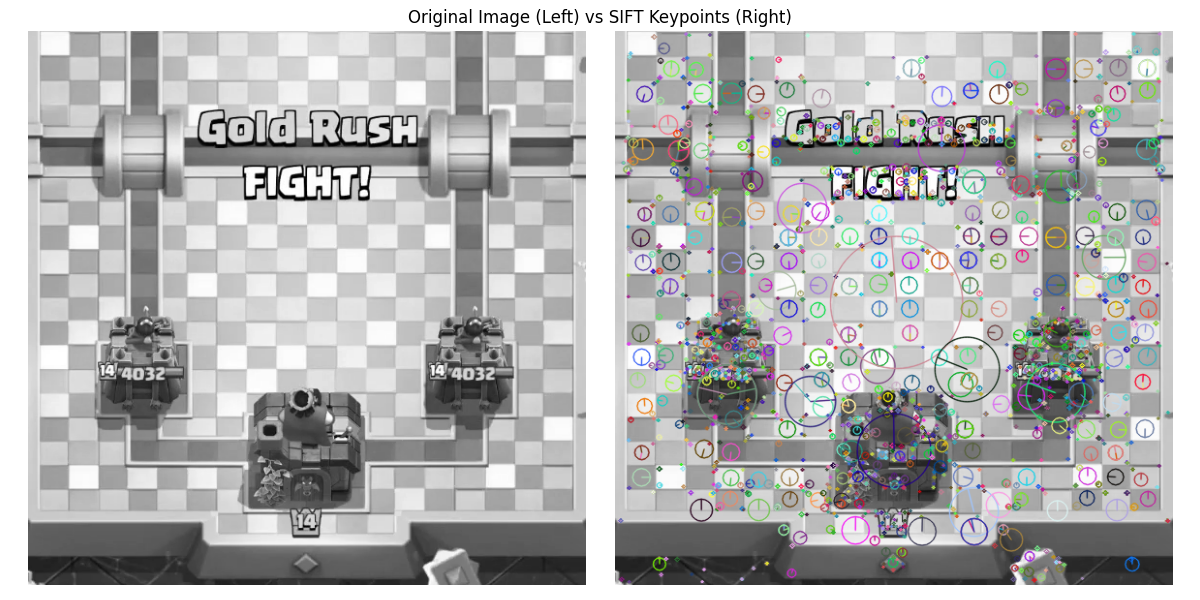
\includegraphics[width=\linewidth]{../code/results/1.png}
    \caption{左图灰度原图,右图SIFT关键点结果}
\end{figure}
\subsection{特征描述子匹配和 RANSAC 方法}
\vspace{3ex}
\begin{pythoncode}
# 1. 初始化 SIFT 检测器
sift = cv2.SIFT_create()

# 2. 检测关键点并计算描述子
keypoints1, descriptors1 = sift.detectAndCompute(image1, None)
keypoints2, descriptors2 = sift.detectAndCompute(image2, None)

# 3. 使用 FLANN(快速近似最近邻) 匹配描述子, 使用 KD 树算法快速匹配描述子
flann_index_kdtree = 1
index_params = dict(algorithm=flann_index_kdtree, trees=5)
search_params = dict(checks=50)

flann = cv2.FlannBasedMatcher(index_params, search_params)
matches = flann.knnMatch(descriptors1, descriptors2, k=2)

# 4. 距离比筛选(Lowe's Ratio Test)
good_matches = []
for m, n in matches:
    if m.distance < 0.7 * n.distance:  # 距离比阈值
        good_matches.append(m)

# 5. 提取匹配点
src_pts = np.float32([keypoints1[m.queryIdx].pt for m in good_matches]).reshape(-1, 1, 2)
dst_pts = np.float32([keypoints2[m.trainIdx].pt for m in good_matches]).reshape(-1, 1, 2)

# 6. 使用 RANSAC 方法估计单应性矩阵
H, mask = cv2.findHomography(src_pts, dst_pts, cv2.RANSAC, 5.0)
matches_mask = mask.ravel().tolist()

# 7. 可视化匹配结果
draw_params = dict(matchColor=(0, 255, 0),  # 内点为绿色
                   singlePointColor=(255, 0, 0),  # 关键点为蓝色
                   matchesMask=matches_mask,  # 仅显示内点
                   flags=cv2.DrawMatchesFlags_DEFAULT)

result_image = cv2.drawMatches(image1, keypoints1, image2, keypoints2, good_matches, None, **draw_params)
\end{pythoncode}
\begin{figure}[htbp]
    \centering
    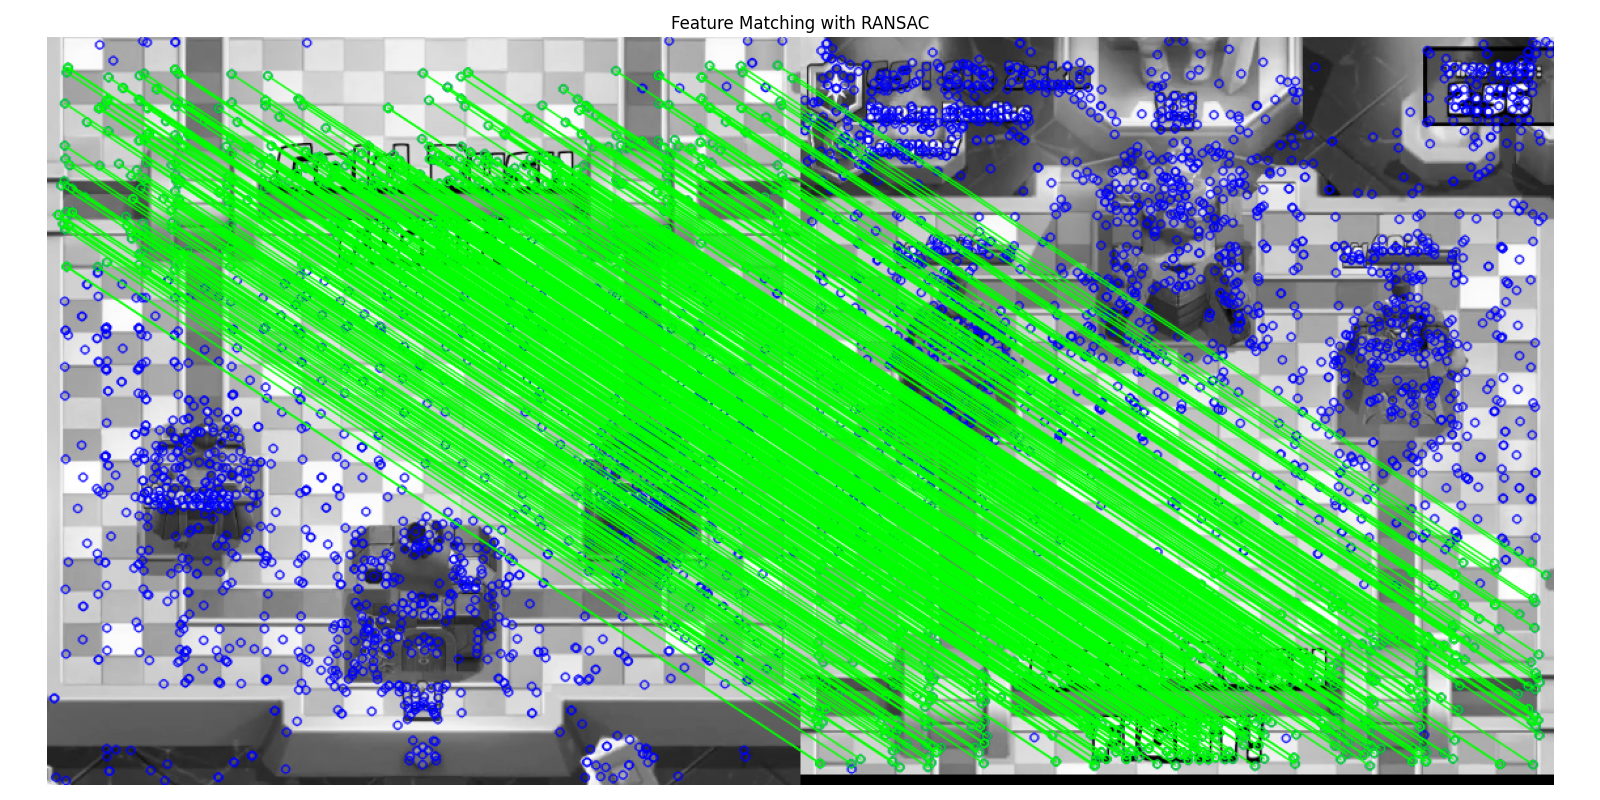
\includegraphics[width=\linewidth]{../code/results/2.png}
    \caption{特征描述子匹配效果(两幅类似背景的图片,在不同时刻下不同位置处的截图)}
    \label{lab-fig2}
\end{figure}

\subsection{图像融合}
\vspace{3ex}
\begin{pythoncode}
# 基于RANSAC得到的单应性矩阵H
# 将第一张图像进行单应性变换,配准到第二张图像,计算输出图像的大小(可以容纳两张图像)
result = cv2.warpPerspective(image1, H, (width + image1.shape[1], height))

# 将第二张图像放入结果图像中
result[0:height, 0:width] = image2

# 在第二张图像(image2)周围画一个绿色的矩形框
cv2.rectangle(result, (0, 0), (width, height), (0, 255, 0), 5)

# 对第一张图像的四个角点应用单应性变换,得到变换后的矩形框
pts = np.float32([[0, 0], [image1.shape[1], 0], [image1.shape[1], image1.shape[0]], [0, image1.shape[0]]]).reshape(-1, 1, 2)
pts_transformed = cv2.perspectiveTransform(pts, H)

# 在变换后的图像中画出第一张图像的矩形框(蓝色)
pts_transformed = np.int32(pts_transformed)
cv2.polylines(result, [pts_transformed], isClosed=True, color=(255, 0, 0), thickness=5)
\end{pythoncode}
\begin{figure}[htbp]
    \centering
    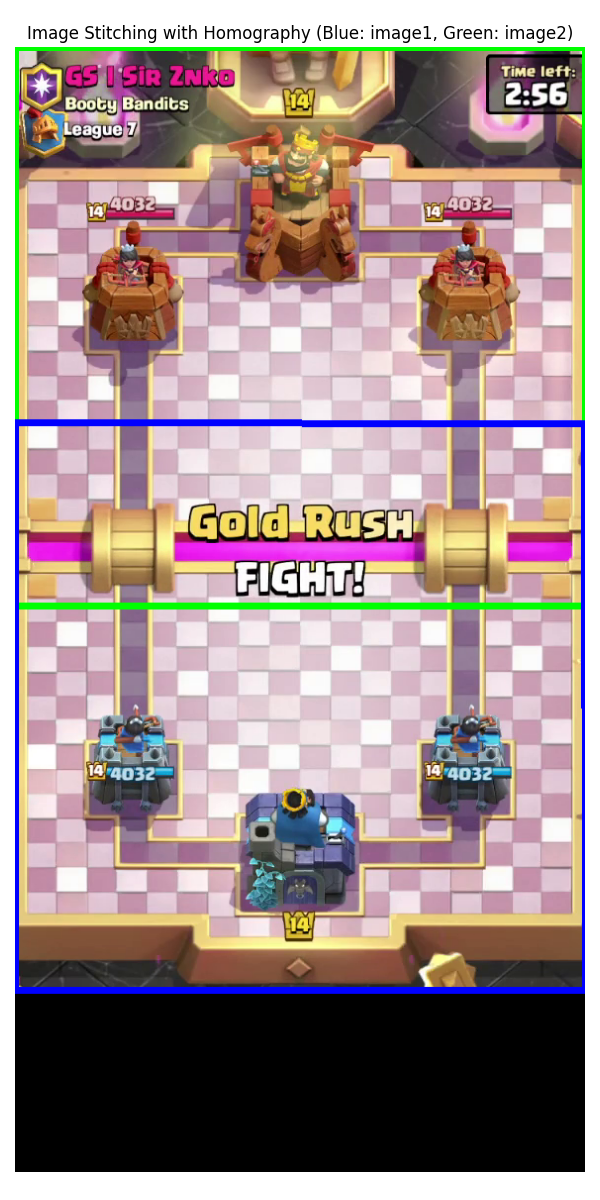
\includegraphics[scale=0.5]{../code/results/3.png}
    \caption{图像融合结果,蓝色为图\ref{lab-fig2}中的左图,绿色为图\ref{lab-fig2}中的右图}
\end{figure}

\end{document}
